\section{The impact of the material budget}\label{sec:impactOfMaterialBudget}

The double\_spirals\_v2 geometry is a more realistic version of the double\_spirals geometry which takes into account the material used for the mechanical support of the sensors and also the material used for the powering of the chip. The material budget per double layer is 0.4\%~X$_{0}$.
The flavor-tagging performance of this geometry is given in Figure \ref{fig:heavy_200} and compared to the double\_spirals. Dijet events with a mixture of angles are used for the flavour tagging.\\
Indeed, by increasing the material in the vertex detector, the performance of the flavour tagging decreases by up to 40\%.


\begin{figure}[H]
        \begin{subfigure}[b]{0.5\textwidth}
          \centering
          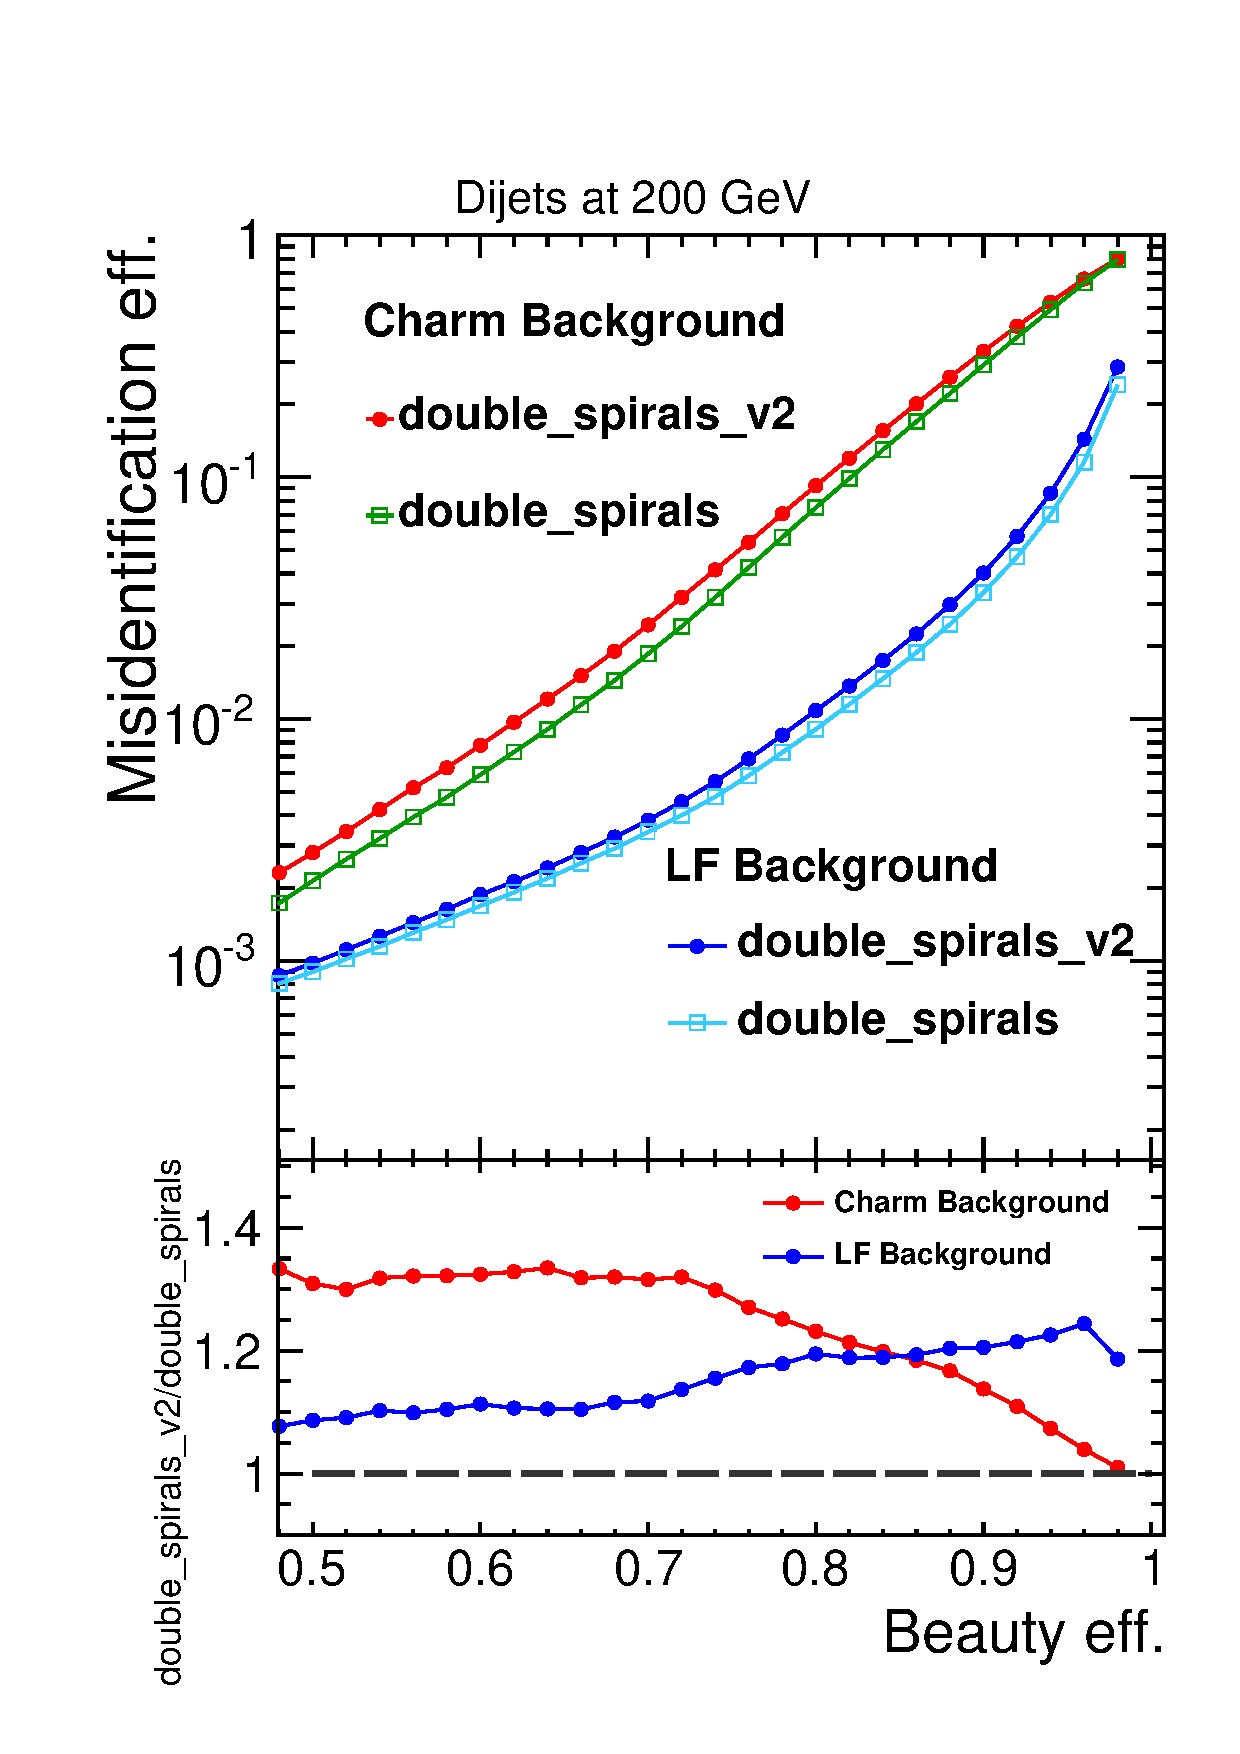
\includegraphics[width=\textwidth]{Figures/ImpactOfGeometries/heavy_general_200_Beauty.pdf}
          \caption{}
          \label{}
        \end{subfigure}%
        ~ 
        \begin{subfigure}[b]{0.5\textwidth}
          \centering
          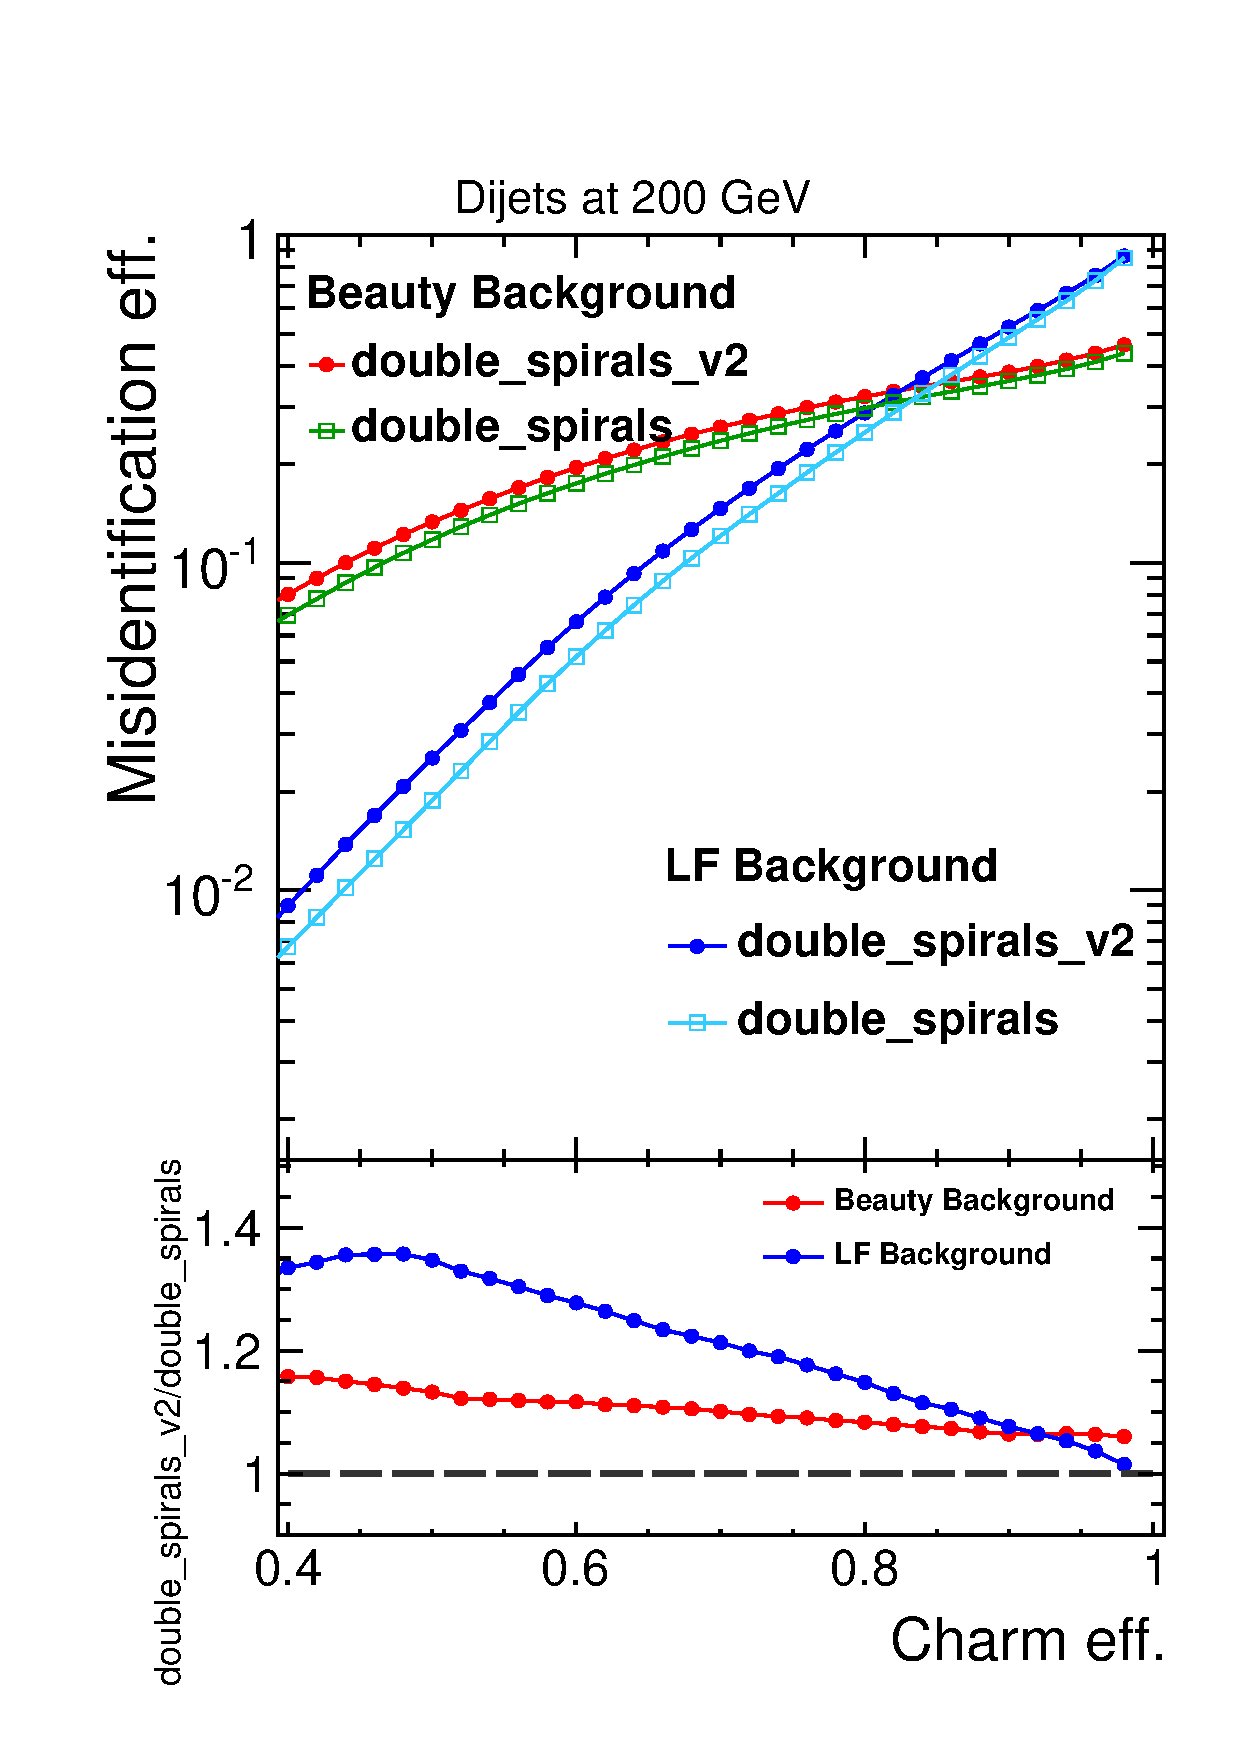
\includegraphics[width=\textwidth]{Figures/ImpactOfGeometries/heavy_general_200_Charm.pdf}
          \caption{}
          \label{}
        \end{subfigure}
        \caption{Global comparison}\label{fig:heavy_200}
\end{figure}
